
%(BEGIN_QUESTION)
% Copyright 2012, Tony R. Kuphaldt, released under the Creative Commons Attribution License (v 1.0)
% This means you may do almost anything with this work of mine, so long as you give me proper credit

Sketch the necessary tube connections to build a working pneumatic temperature-control loop, maintaining the oil at a constant temperature as it exits the heat exchanger.  One of the pneumatic control valves needs to be positioned by pressure from the manual regulator, while the other needs to be controlled by the temperature controller (TIC-51).  Note the three shut-off valves, each one intended to provide a source of instrument air to each of the three field instruments:

$$\includegraphics[width=15.5cm]{i01916x01.eps}$$

Assume the temperature transmitter (TT-51) is direct-acting, and that the pneumatic controller (TIC-51) is only capable of {\it reverse action} and cannot be set for direct action.

\underbar{file i01916}
%(END_QUESTION)





%(BEGIN_ANSWER)

10 points, all or nothing.  While there may be valid variations for how to plumb the air supply lines, the other lines must go where they are shown in order for the system to work at all (i.e. hand regulator to oil valve, controller output to steam valve, transmitter output to controller input):

$$\includegraphics[width=15.5cm]{i01916x02.eps}$$

%(END_ANSWER)





%(BEGIN_NOTES)

{\bf This question is intended for exams only and not worksheets!}.

%(END_NOTES)


